\documentclass[11pt,a4paper]{article}
\usepackage[margin=2.2cm]{geometry}
\usepackage{graphicx,amsmath,amssymb,booktabs,xcolor,hyperref,float,caption,array}
\newcommand{\kT}{k_BT}\newcommand{\half}{\tfrac12}\newcommand{\la}{\ell_a}
\setlength{\parskip}{4pt}\setlength{\parindent}{0pt}
\title{Elastic anisotropy and site selection in MPCD cavities}
\author{Findings of 20--22 October 2026}
\date{}
\begin{document}\maketitle

\section*{Summary}
\begin{enumerate}
\item \textbf{The splay--bend anisotropy of 2D MPCD comes from the flow coupling.} With the director--flow coupling off, the fluctuation spectrum
is isotropic, $K_1=K_3=43.8\,\kT$, as Shendruk \& Yeomans (2015) found in 3D with the same switch. With it on, $K_1/K_3$ follows the
flow-alignment parameter: 0.49, 1.05, 1.49 and 1.97 at $\lambda=-2$, 0, 1 and 2.
\item \textbf{The defects do not feel it.} The static response of the director to a field is close to isotropic at every scale tested (3--18
cells): $K_1/K_3\approx0.81\pm0.07$ with the coupling on, $0.96\pm0.05$ off. The coupling makes the \emph{noise} anisotropic (bend modes are
driven harder by thermal velocity gradients); the stiffness stays isotropic, $K\approx44\,\kT$.
\item \textbf{Site selection needs no anisotropy.} The wall defects of active cavities sit at the same positions for every initial condition
because the flow fixes the common tilt ($\arccos(1/\lambda)$) and the tilt--position lock fixes the registry. The one-constant continuum model does
the same (registry offset 0.01--0.24\,rad, MPCD 0.03), and passive layers switched to active all end at the same registry, whatever registry
they started from.
\item \textbf{Elasticity enforces the lock; the flow chooses the point on it.} With orientation treated as a slow variable, the one-constant energy
is flat along the lock and stiff across it (twist stiffness 24--28\,$\kT$/rad$^2$ per defect for sparse layers, 12 at $k=16$).
\item \textbf{One correction to the tilt analysis.} MPCD multiplies the Jeffery rotation by the shear susceptibility $\chi_\mathrm{HI}=0.5$; the
MPCD alignment length omitted it (too short by $\sqrt2$) and used $K=32.5$ instead of 44: $\ell_E$ is about 1.65 times longer, and $d/\ell_E$
of MPCD cores is 0.3--0.7 instead of 0.5--1.2.
\end{enumerate}
What survives unchanged: the lock and the $2|k-1|$ count, the tilt law $\arccos(1/\lambda)$, every measured observable, and the signs and ratios
of the ejection and shielding energetics. What changes: the mechanism quoted for site pinning (80--110\,$\kT$ from $K_1\neq K_3$), the
attributions ``elasticity alone gives $35^\circ$'' and ``$+2$--$3^\circ$ from splay $\neq$ bend'', the static elastic pull invoked for the crowding
drop, and the quoted constants. The claim-by-claim survey is reports/frank\_survey.

\section{The fluctuation constants depend on the flow coupling}
MPCD rotates each particle's orientation by Jeffery's equation, scaled by the shear susceptibility $\chi_\mathrm{HI}$ (code default 0.5, our
production value), with flow-alignment parameter $\lambda$ (production 2). Thermal velocity fluctuations therefore keep rotating the director.
For a director along $x$, $\dot\theta=\chi_\mathrm{HI}[\tfrac12(1+\lambda)\partial_xv_y-\tfrac12(1-\lambda)\partial_yv_x]$: bend modes are driven
with weight $(1+\lambda)/2$, splay modes with $(1-\lambda)/2$. At $\lambda=2$ bend is driven about nine times harder in power, which reads as a
softer $K_3$ in an equipartition fit. Shendruk \& Yeomans measured their isotropic constants with the coupling off ($w_\mathrm{HI}=0$, their
Fig.~7); our calibration had it on.

\begin{table}[H]\centering\small
\begin{tabular}{lccc}\toprule
Passive $64^2$ box, 2 seeds & $K_1$ (splay) & $K_3$ (bend) & $K_1/K_3$\\\midrule
Coupling off ($\chi_\mathrm{HI}=0$) & 43.7, 44.0 & 43.5, 43.9 & 1.00--1.01\\
$\lambda=0$ & 39.0, 39.3 & 37.1, 37.6 & 1.04--1.06\\
$\lambda=1$ & 43.5, 44.1 & 29.2, 29.5 & 1.47--1.51\\
$\lambda=2$ (production) & 42.8, 43.1 & 21.7, 22.0 & 1.96--1.97\\
$\lambda=-2$ & 21.1, 21.2 & 43.5, 43.6 & 0.48--0.49\\\bottomrule
\end{tabular}
\caption{Fluctuation constants ($\kT$), director-frame maximum-likelihood fits over $0<|q|<0.8$. $\langle S\rangle=0.876$--0.877 in all.}
\end{table}
A mode with zero coupling keeps the bare value ($K_1$ at $\lambda=1$); $\lambda\to-\lambda$ swaps splay and bend (rod--disc symmetry of the
Jeffery term). Checks: the fits converge from different starting points, the small-angle expansion holds (dropped terms 1--2\% of the power),
and with the coupling off the spectrum has no $q$-dependence. The rotational viscosity from mode decay is unchanged with the coupling off,
$\gamma_1\approx60$.
\begin{figure}[H]\centering
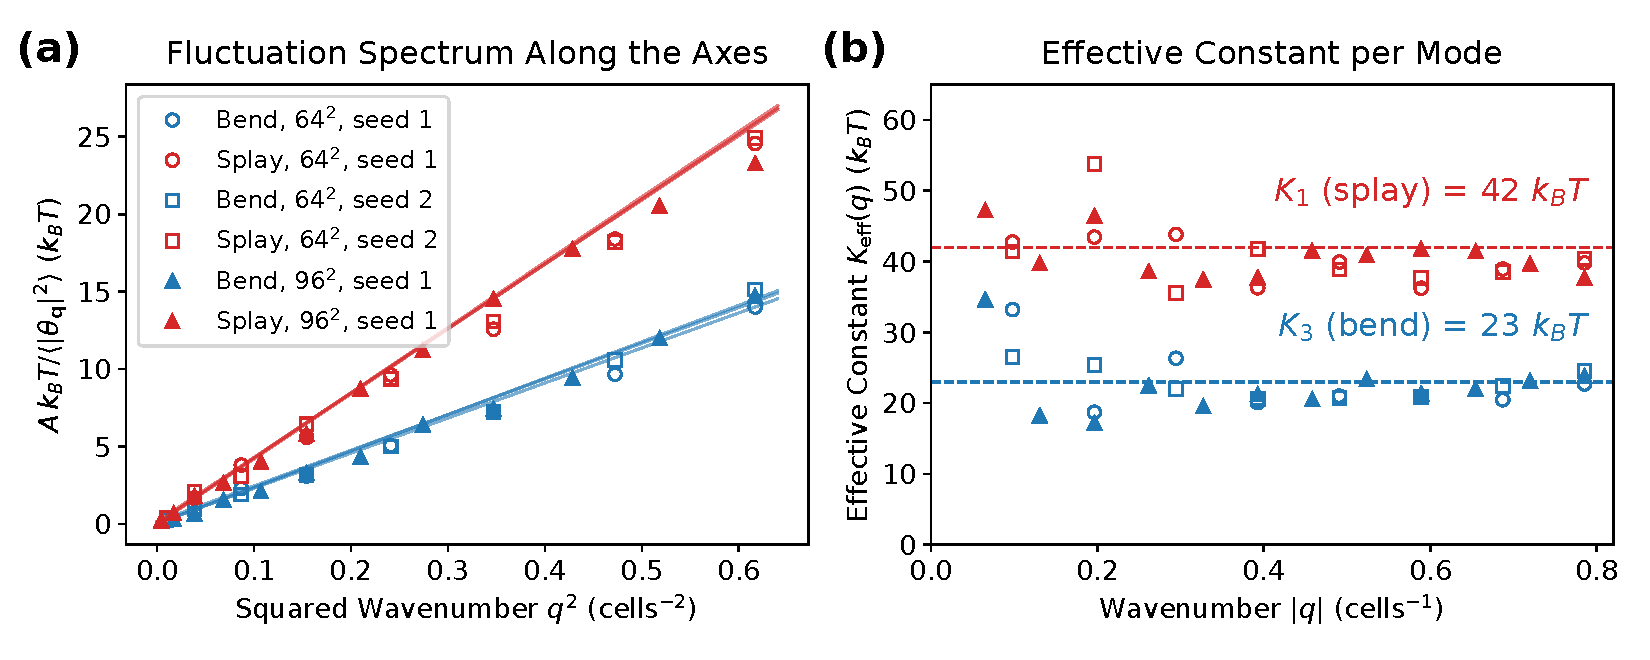
\includegraphics[width=0.49\textwidth]{../master/figs/frank_spectrum.pdf}\hfill
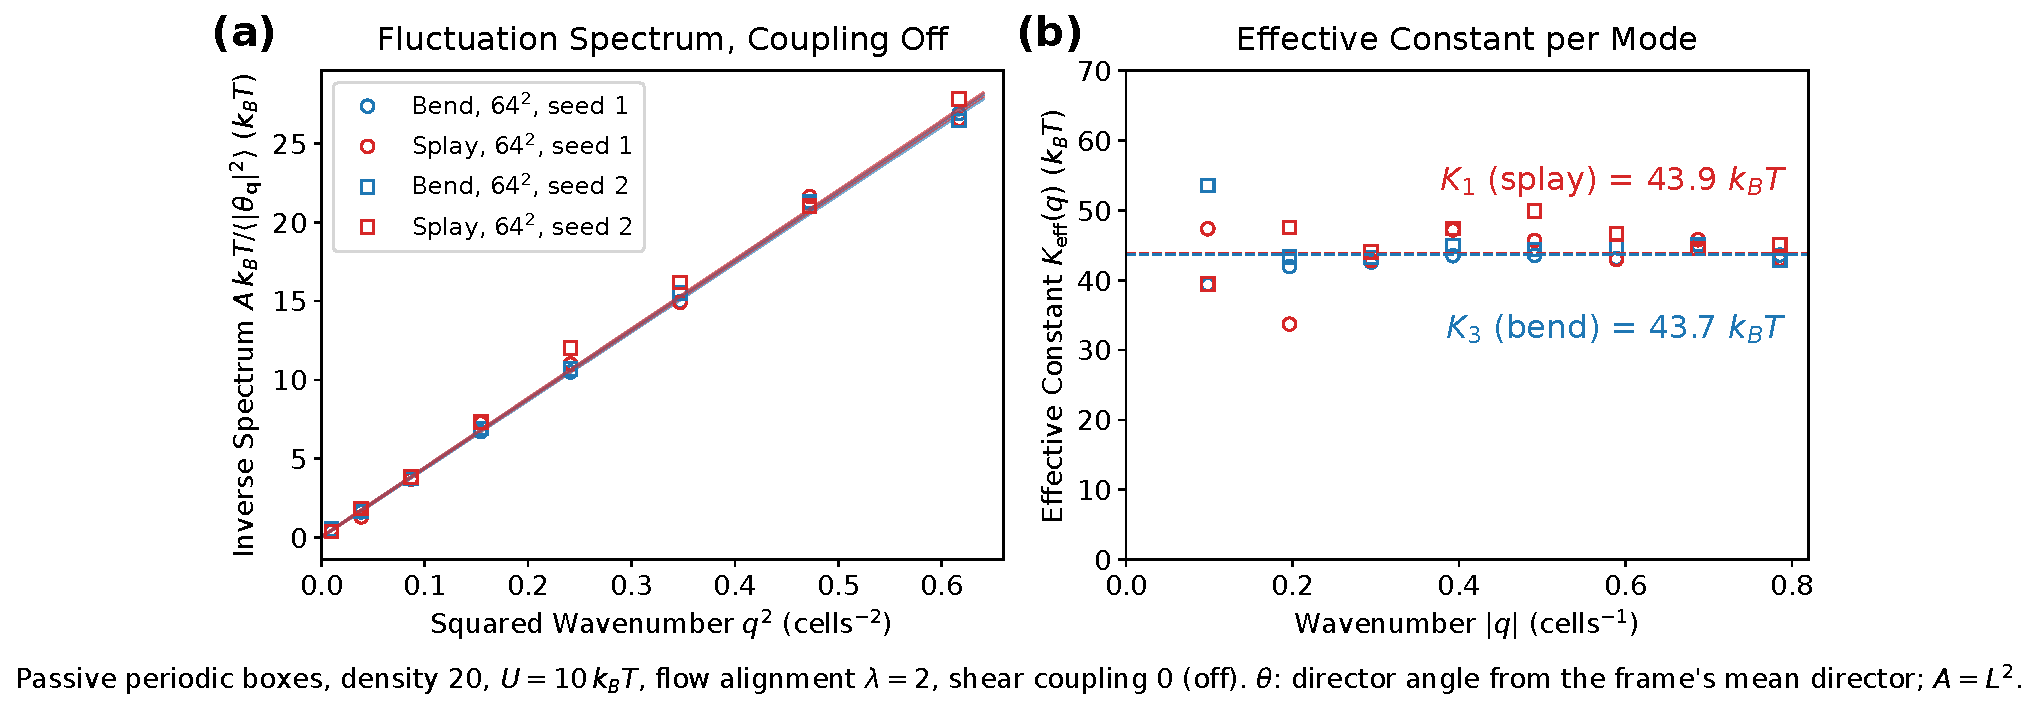
\includegraphics[width=0.49\textwidth]{../master/figs/frank_spectrum_nocoupling.pdf}
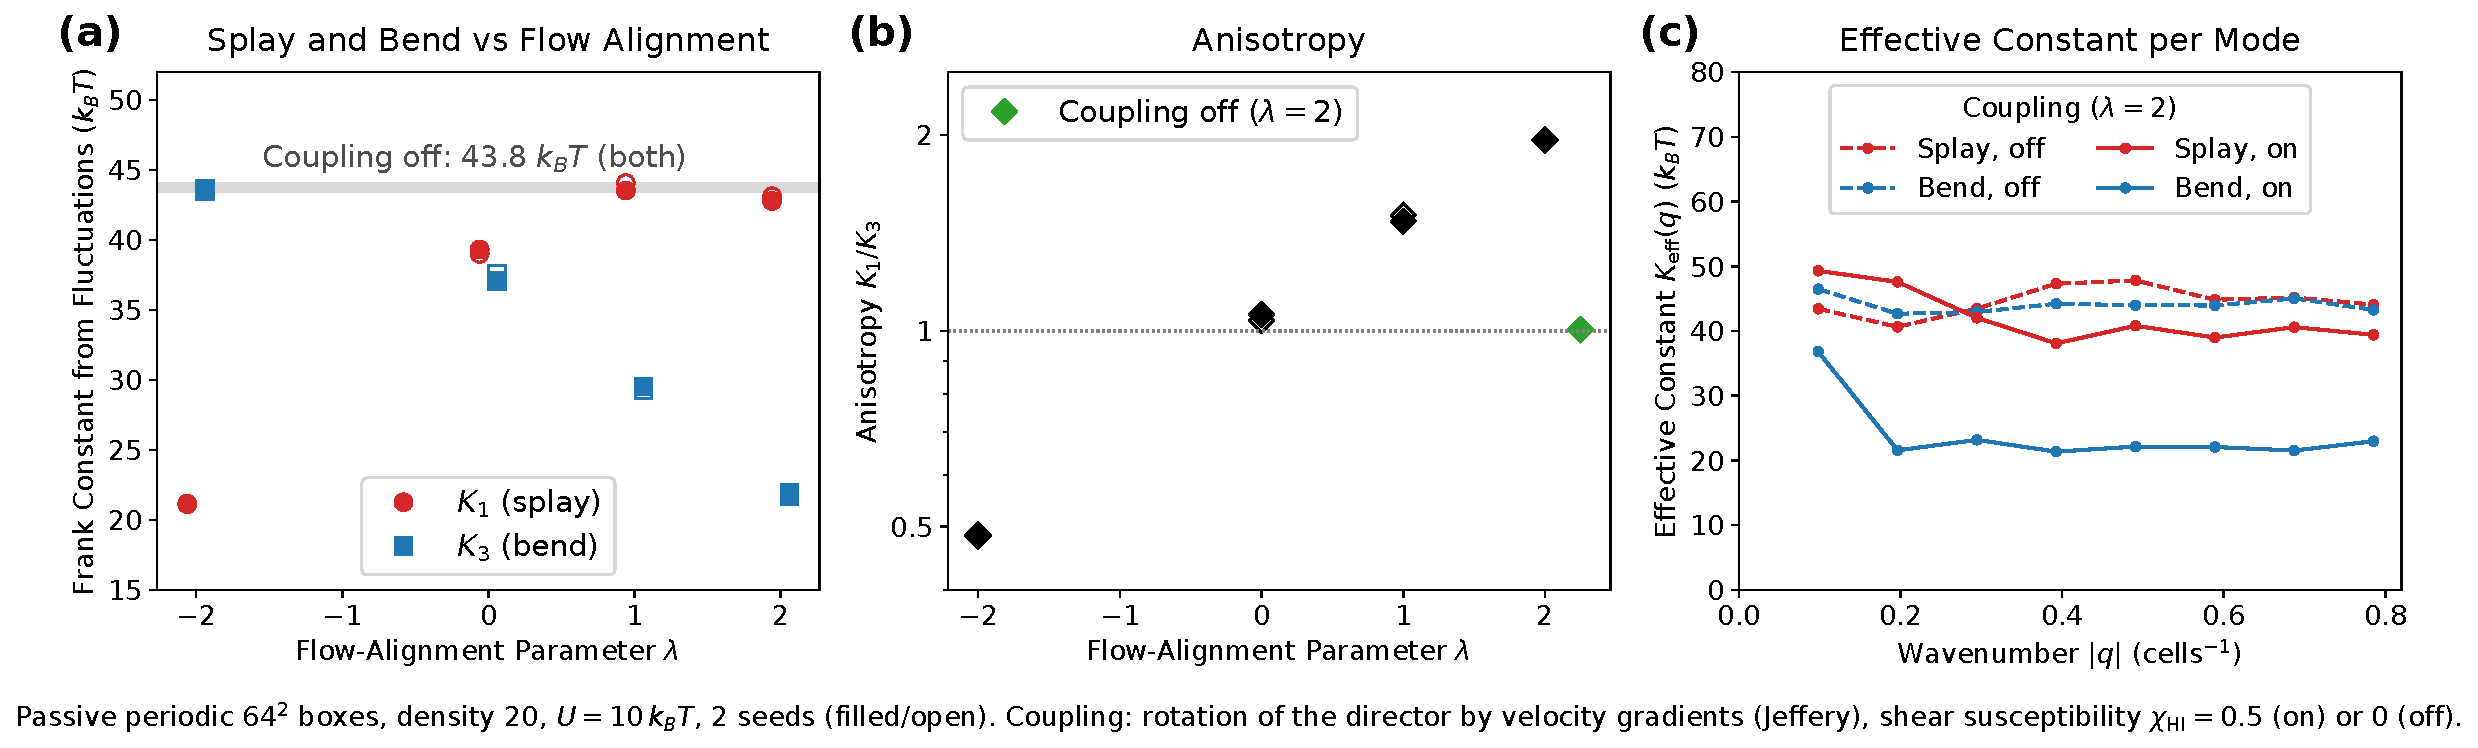
\includegraphics[width=\textwidth]{../master/figs/frank_coupling.pdf}
\caption{Top: fluctuation spectra in the director frame with the coupling on (left) and off (right). Bottom: the constants and their ratio
against $\lambda$, and the effective constant per mode with the coupling off and on.}
\end{figure}

\section{The static response is isotropic}
Fluctuations measure $K/T_\mathrm{eff}$ per mode; what shapes defects is the stiffness in the response to a static torque. In a passive channel
with planar walls (director along the wall) or homeotropic walls (normal to it), a weak field tilted $10^\circ$ from the wall axis pulls the bulk
director; the time-averaged profile heals from the wall over $\xi\propto\sqrt{K/(\text{field})}$, with splay in the planar case and bend in the
homeotropic one. The same field in both gives $K_1/K_3=(\xi_\mathrm{splay}/\xi_\mathrm{bend})^2$, with no equipartition assumption.
\begin{table}[H]\centering\small
\begin{tabular}{lcc}\toprule
Channel width, field (healing length $\xi$) & coupling off & coupling on ($\lambda=2$)\\\midrule
40, $H=8$ (6--9 cells) & $1.38\pm0.35$ & $0.94\pm0.16$\\
40, $H=12$ (4.5--5.5) & $0.96\pm0.12$ & $0.79\pm0.18$\\
40, $H=16$ (3.2--3.9) & $0.93\pm0.06$ & $0.74\pm0.15$\\
80, $H=4$ (12--18; 3 seeds on, 2 off) & $1.11\pm0.35$ & $0.82\pm0.18$\\
80, $H=6$ (9--14; 3 seeds) & -- & $0.77\pm0.15$\\\bottomrule
\end{tabular}
\caption{Response $K_1/K_3$ (fits with the bulk angle at the field angle; errors from time blocks and seeds). $\xi\propto1/H$ as estimated.}
\end{table}
The factor 2 of the fluctuations is absent from the response. A small difference between coupling on ($\approx0.8$) and off ($\approx1$) is at
the $2\sigma$ level, has the opposite sign to the fluctuation anisotropy, and may be a fit systematic. The splay/bend difference in mode decay
rates (1.2--1.5 with the coupling on) is then a friction (backflow) effect.

\section{Site selection by the flow through the lock}
\textbf{The observation.} In active cavities the wall defects end at the same positions relative to the anchoring for every initial condition:
the homeotropic sites shifted by $\tau/(2k-2)$, with only the chirality spontaneous (lock-corrected registry $D=0.03\pm0.07$, 8 runs from 6
initial directors). With a modulated anchoring they follow the moved sites. We had attributed this to an elastic barrier from $K_1\neq K_3$.

\textbf{The explanation without anisotropy.} (1) The lock: with one Frank constant, sliding a wall defect by $D$ rotates its far field, so the
registry offset equals $\tau/(2k-2)$; the sites are fixed by the anchoring. (2) The no-slip shear at the wall turns the far field to the
flow-aligned angle, $\tau=\arccos(1/\lambda)\approx63^\circ$, with the sign of the circulation. (3) Once the flow fixes $\tau$, the lock fixes every
position. At rest all registries cost the same; without flow the registry stays where the initial condition left it, as observed in passive
cavities (registry set by the initial director, seeded tilts of 60 and $120^\circ$ kept for hundreds of t.u.).

\textbf{The continuum does the same.} With the MPCD estimator on every one-constant continuum disk (activity $\zeta=3$--8 and imposed-swirl
controls; same anchoring), the layers with $2k-2$ wall defects sit at the lock position: $D=0.01$--0.24\,rad, $|Z|=0.98$--1.00, arg
$Z\approx\pm1.1$\,rad for tilts of 51--$65^\circ$, both chiralities. The model has no anisotropy, so site selection is not an MPCD peculiarity.

\textbf{The lock valley.} Rigid cores of prescribed orientation, Frank field relaxed outside (circle $R=31.8$, ring of $2k-2$ plus a central
$+1$), give the energy as a function of the registry shift and the core orientation (Fig.~\ref{fig:valley}). With one constant ($K=44$) it is a
valley, flat along the lock to within 1--1.5\,$\kT$ per defect (grid) and stiff across it: a $30^\circ$ twist off the lock costs 2--4\,$\kT$ per
defect, $60^\circ$ 6--16. A $63^\circ$ tilt made by rotating cores in place would cost 10--20\,$\kT$ per defect; made by sliding along the valley it
costs nothing. The twist stiffness softens with crowding (24--28 at $k=4$--6, 12 at $k=16$). With the fluctuation anisotropy imposed instead
(43.1/21.9), the valley acquires a floor at zero tilt (6--8\,$\kT$ per defect at $180^\circ$): the barrier we had quoted, now not supported by the
response.
\begin{figure}[H]\centering\includegraphics[width=0.8\textwidth]{../master/theory/lockvalley/fig_lock_valley.pdf}
\caption{The lock valley: energy per wall defect against the registry shift (as the lock tilt) and the orientation offset, $k=6$, one constant
(a) and imposed anisotropy (b); (c) along the lock for $k=4$--16; (d) twist stiffness across the lock.}\label{fig:valley}\end{figure}

\textbf{Crowded walls: the shift follows the tilt} (Fig.~\ref{fig:shift}; theory/lockshift). Crowded walls tilt less, and $\lambda$ changes the
tilt at fixed crowding, so the predicted shift of the defects from the homeotropic points changes with them. Over 1454 active runs of the main sweep
(spacing 50 to 4 cells, tilt from $\approx30$ to $70^\circ$), (shift)$\times(2k-2)$ follows the tilt with slope 1.00: in the most crowded walls
(spacing $<8$) the tilt is $44^\circ$ and the shift corresponds to $49.6^\circ$, against $64.4$ and $64.9^\circ$ for spacing $>20$. A shift frozen at
the sparse value is ruled out. Passive layers under an imposed vortex and the $\lambda$ scans at $k=6$ and 14 (tilt 47--$78^\circ$ at fixed
crowding) follow the same line. A small constant offset remains, $+4$--$5^\circ$ in (shift)$\times(2k-2)$ for spacing below 20 (about 0.1 cell
along the wall), decreasing to $\approx0$ or slightly negative in the sparsest walls.

\textbf{Is the offset a tracking artefact?} Statistical errors are small (bootstrap standard error of the median 0.1--$0.25^\circ$ per spacing
bin; per-run scatter 2--$3^\circ$). Systematic errors were tested two ways (theory/trackerr). (1) Seeded layers with known positions and tilts
(runs/rest\_pinning, first frames): the tracker's error in (shift$\times(2k-2)$ $-$ tilt) is $+3.5\pm4.0$, $+0.4\pm2.2$, $-0.4\pm2.2$ and
$-2.5\pm1.4^\circ$ at spacing 32, 19, 11 and 6 cells; positions are unbiased to within 0.1 cell. (2) Real frames (39 runs): re-locating each wall
defect with sub-cell precision from the order-parameter field changes the offset by less than $1^\circ$ (e.g.\ $+5.1\to+4.0^\circ$ at spacing 8--12),
and measuring the tilt independently from $\nabla\cdot Q$ restores it ($+4.8^\circ$); the tracked core centre sits only 0.04--0.09 cells along the
comet axis from the refined one. Tracking accounts for at most $\approx1$--$2^\circ$ of the $+4$--$5^\circ$, with no consistent sign, so a small real
offset remains: in walls with spacing below 20 cells the defects sit about 0.1 cell further along the wall than the tilt alone predicts.
\begin{figure}[H]\centering\includegraphics[width=0.9\textwidth]{../master/theory/lockshift/fig_lock_shift.pdf}
\caption{(a) Position shift of the wall defects from the homeotropic points (times $2k-2$) against the tilt, one point per run; dashed: the
prediction; dotted: a shift frozen at the sparse value. (b) Deviation from the prediction against the wall-defect spacing.}\label{fig:shift}\end{figure}

\textbf{Passive $\to$ active switch} (Fig.~\ref{fig:switch}; movies in theory/switchon/movie). Eight passive cavities ($k=6$, 12 wall defects,
registries frozen by eight initial directors, arg $Z_{12}$ from $-1.73$ to $+1.16$) were resumed with activity 0.07. All eight end at the registry
of cavities that were active from the start: arg $Z_{10}=\pm1.16$--1.18, $|Z|=1.00$, $D=\pm0.06$--0.07, tilt 63--$65^\circ$, circulation
0.86--0.96 (five of one sign, three of the other). The passive registry is not slid into place but erased: activity first melts the layer (12
$\to$ 2--4 wall defects within $\approx50$\,t.u.), the coherent flow builds over 200--800\,t.u., the tilt settles once the circulation passes
$\approx0.6$, and the wall refills to 10 at the flow-selected registry.
\begin{figure}[H]\centering\includegraphics[width=0.8\textwidth]{../master/theory/switchon/fig_switchon.pdf}
\caption{Passive $\to$ active switch: wall count, circulation, tilt and registry against time, eight initial conditions.}\label{fig:switch}\end{figure}

\section{The alignment length}
The boundary-layer analysis of the tilt uses $\ell_E=\sqrt{K/(\gamma_1 s\sqrt{\lambda^2-1})}$. In MPCD the flow torque per $\gamma_1$ is scaled by
$\chi_\mathrm{HI}$, so $\ell_E=\sqrt{K/(\chi_\mathrm{HI}\gamma_1 s\sqrt{\lambda^2-1})}$. With $K=44$ and $\chi_\mathrm{HI}=0.5$ the MPCD alignment length is
2.3--4.4 cells (was 1.4--2.7), and the core depths are $d/\ell_E\approx0.3$--0.7 (was 0.5--1.2). The ordering of the crowding drop by $d\sqrt s$ is
unaffected (a uniform rescaling), but the statement that the continuum activity scan ``brackets'' the MPCD range no longer holds: MPCD sparse layers
sit near the continuum's crowded value. The boundary-layer ansatz estimate ($+16^\circ$, which already included $\chi_\mathrm{HI}$) becomes $\approx14^\circ$,
still far above the measured 2--4$^\circ$.

\section{Consequences and open points}
\begin{itemize}
\item \textbf{Paper text.} Quote $K\approx44\,\kT$ (isotropic; the coupled fluctuation constants as a property of the noise); replace ``pinning
by splay $\neq$ bend'' with ``site selection by the flow through the lock''; drop the $35^\circ$ and $+2$--$3^\circ$ attributions (the one-constant
flat wall gives 61--$69^\circ$, against 62--$64^\circ$ measured); recompute one-constant energies at $K=44$ (ratios unchanged); include
$\chi_\mathrm{HI}$ in $\ell_E$. Sections affected: SI S1, S5, S7--S8; about three PRL sentences.
\item \textbf{Open: the stiffness of the selected registry.} The collective registry fluctuates by 0.29--0.36 cells. In the lock + flow picture this
is set by the flow-alignment torque through the boundary layer, which the flat-wall continuum model can estimate.
\item \textbf{Open: the crowding drop.} Without a static elastic pull, the restoring torque that makes crowded layers tilt less must be dynamic.
The twist stiffness softening with crowding (lock held less firmly) is a candidate; the active one-constant continuum disk, which shows a drop of
8--$11^\circ$, becomes the matching model.
\item \textbf{Open: the activity-scale shift since 2024.} The turbulence onset scales as $K_3/[\chi_\mathrm{HI}(1+\lambda)]$; a change in the flow
coupling between code versions remains a candidate (TODO).
\item \textbf{For Tyler.} The 2015 isotropic constants hold in 2D for the bare elasticity; with the coupling on, the equilibrium fluctuations
of nematic MPCD are anisotropic and set by $\lambda$, while the static response is not.
\end{itemize}
\end{document}
